\section{Results}
\label{sec:results}

We found that our algorithm created trajectories that were free of collisions and produced smooth motion. In Figure~\ref{fig:res:steps} we have a diagram showing the patch in various steps of our algorithm. Next we show the final curved trajectories with various sized input. Lastly we show some performance tests.

\devin{the images are not lining up how I want them too.}
\panayiotis{Devin, I took the liberty of modifying the figures below to show you how its typically done. Note the label for referencing the figures in the text.}

\begin{figure*}[t]
 \centering
 \begin{subfigure}[b]{0.24\linewidth}
 	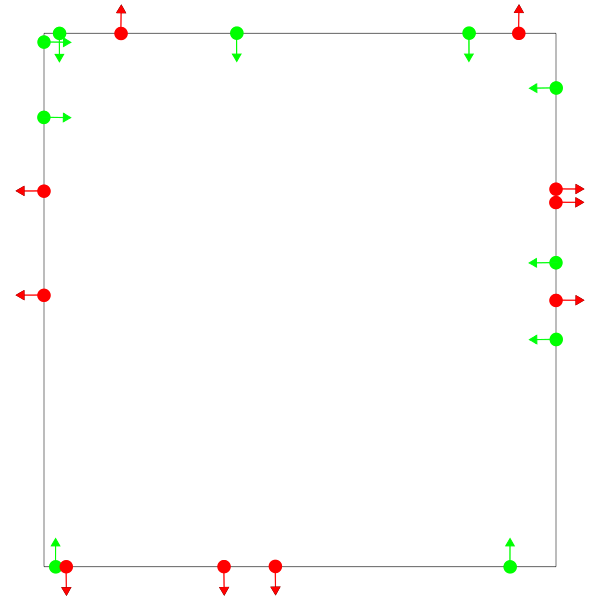
\includegraphics[width=\linewidth]{images/steps-input.png}
 	\caption{Input}
 \end{subfigure}
 % 
 \begin{subfigure}[b]{0.24\linewidth}
 	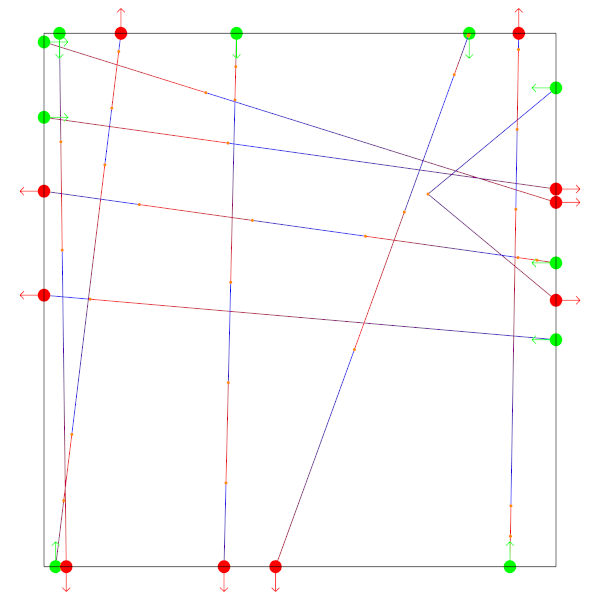
\includegraphics[width=\linewidth]{images/steps-connected.png}
 	\caption{Connected}
 \end{subfigure}
 %
 \begin{subfigure}[b]{0.24\linewidth}
 	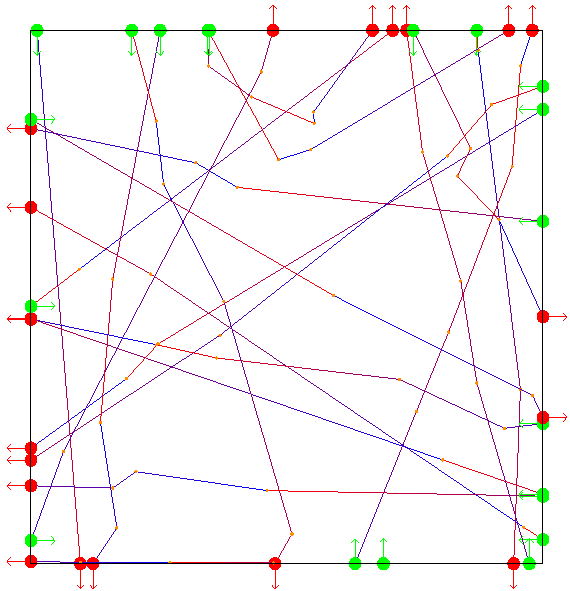
\includegraphics[width=\linewidth]{images/steps-collisionFree.png}
 	\caption{Collision Free}
 \end{subfigure}
 %
 \begin{subfigure}[b]{0.24\linewidth}
 	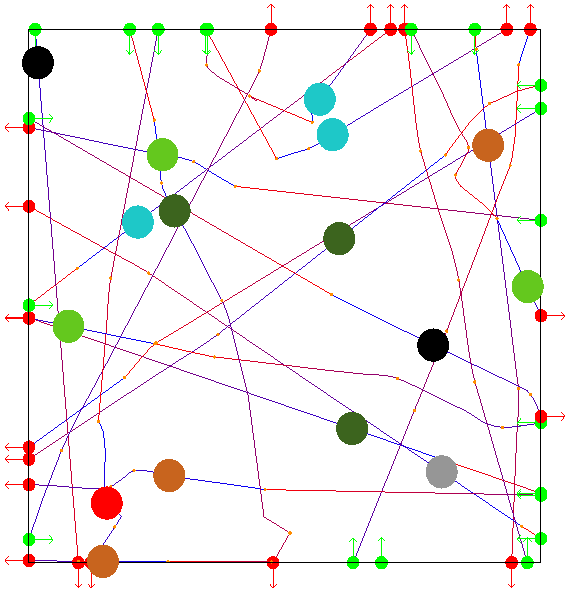
\includegraphics[width=\linewidth]{images/steps-smoothed.png}
 	\caption{Smoothed Out}
 \end{subfigure}
 \caption{Various steps of our algorithm.}
 \label{fig:res:steps}
\end{figure*}


The performance was measured on a computer with an Intel Xeon quad core 2.8 GHz processor and 8GB of RAM. We found trajectories for patches with randomly generated entry and exit points. The patches all had base square of size 16 by 16. The period was 10 seconds. There were 20 samples for each number of agents between 1 and 50 for a total of 1000 samples. 994 of these were collision free. The other 6 were stopped after they reached 2000 iterations. We recorded the number of iterations required for collision free trajectories as well as the computation time in seconds.

\begin{figure*}[t]
 \centering
%
\begin{subfigure}[b]{0.24\linewidth}
	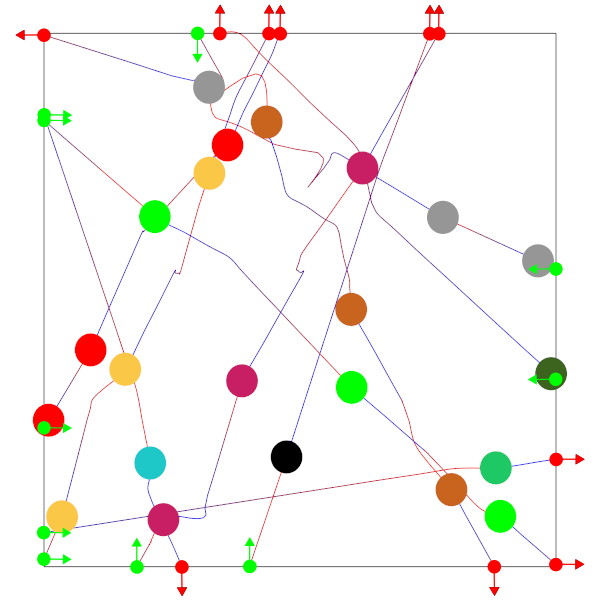
\includegraphics[width=\linewidth]{images/res-10-entry-exit.png}
	\caption{10 Entry/Exit Points}
 \end{subfigure}
%
 \begin{subfigure}[b]{0.24\linewidth}
	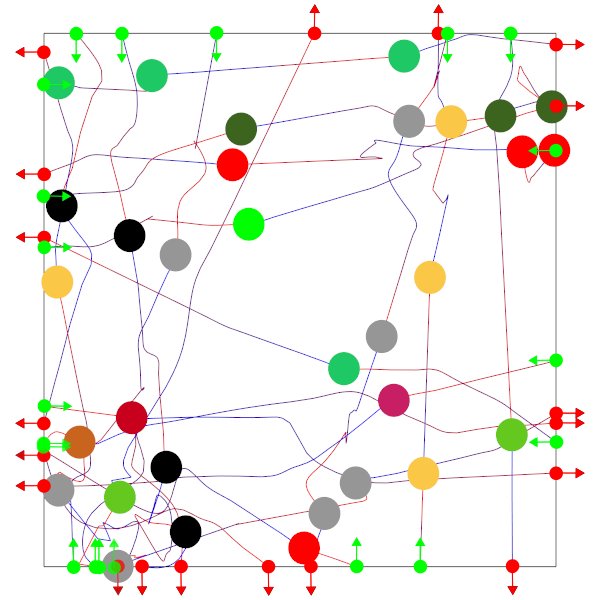
\includegraphics[width=\linewidth]{images/res-20-entry-exit.png}
	\caption{20 Entry/Exit Points}
 \end{subfigure}
%
 \begin{subfigure}[b]{0.24\linewidth}
	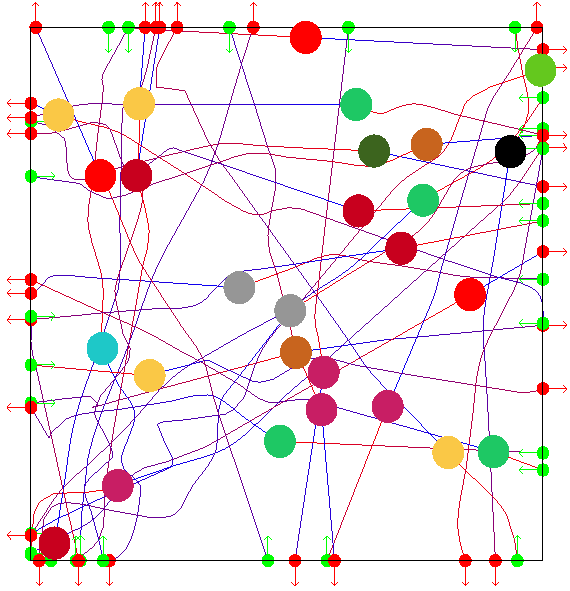
\includegraphics[width=\linewidth]{images/res-30-entry-exit.png}
	\caption{30 Entry/Exit Points}
 \end{subfigure}
%
 \begin{subfigure}[b]{0.24\linewidth}
	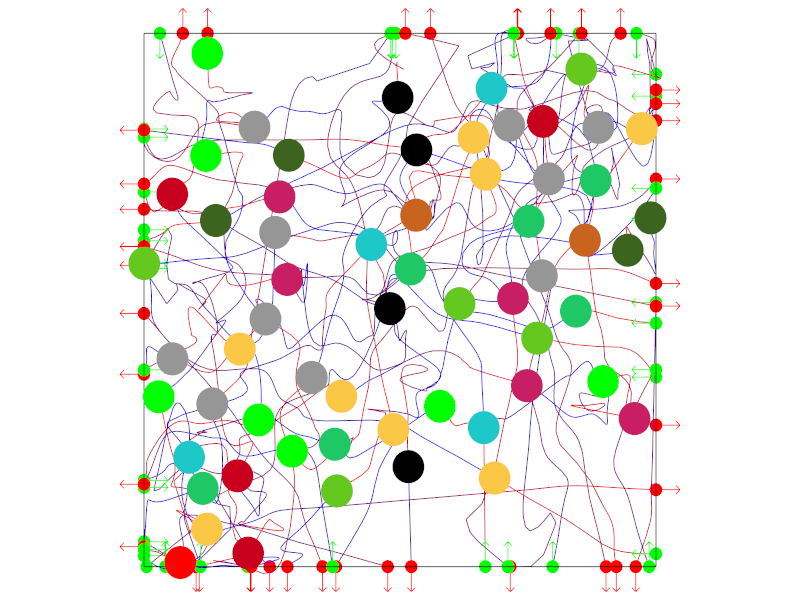
\includegraphics[width=\linewidth]{images/res-40-entry-exit.png}
	\caption{40 Entry/Exit Points}
 \end{subfigure}
%
\caption{Various input to our algorithm.}
\label{fig:res:inputs}
\end{figure*}

\begin{figure*}[t]
 \centering
%
\begin{subfigure}[b]{0.48\linewidth}
 \centering
	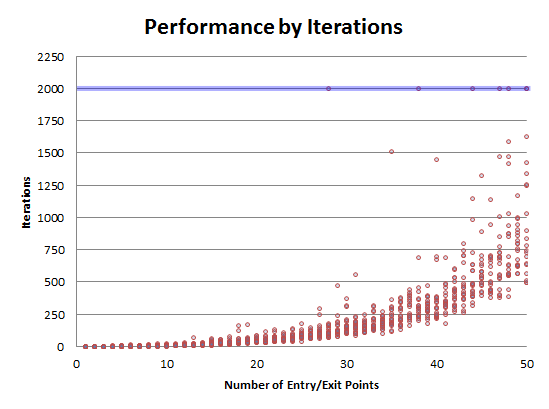
\includegraphics[width=\linewidth]{images/res-iter-graph.png}
	\caption{}
 \end{subfigure}
%
\begin{subfigure}[b]{0.48\linewidth}
 \centering
	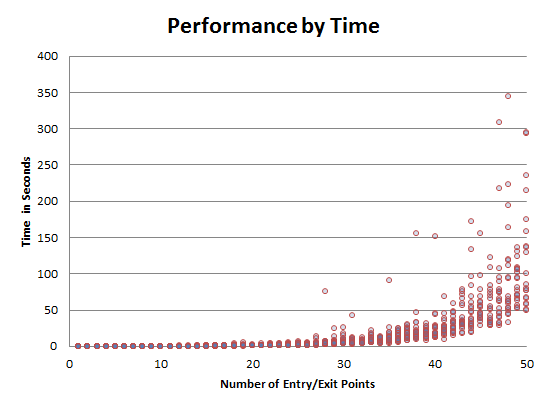
\includegraphics[width=\linewidth]{images/res-time-graph.png}
	\caption{}
 \end{subfigure}
% 
\caption{\textbf{(a)} The dots indicate the number of iterations each experiment needed to converge whereas the blue horizontal line indicates the maximum number of allowed iterations ($6$  out of $1000$ inputs \panayiotis{What do we mean by inputs? experiments or the total number of trajectories. Does this graph show how much time it took for a whole patch or for the trajectories with collisions?} didn't converge after $2000$ iterations) . \textbf{(b)} The time to converge was measured in seconds.  \devin{should I remove the titles on the images of the graphs, and instead put their title in the caption?} \panayiotis{No, you should leave them.. If you can edit the images, please remove the borders. I think it will look nicer. Also, this graphs confuse me a little bit. We should discuss them with Guillermo - I want to get a feeling of what exactly are we showing here\ldots}}
\label{fig:res:graphs}
\end{figure*}
